Many people, I suspect, use the idiom, ``Hindsight is twenty-twenty'' in a way that is better served by other, more appropriate words or phrases.   The sense in which I hear it most commonly used is perhaps more adequately covered by the beautiful portmanteau, ``regretrospect''.  That is, now that things are said and done, I respect a lot of what happened during this adventure.

Also, it's my second favorite portmanteau after ``congratudolences'' and really ought to see wider use.

No, I think ``hindsight is twenty-twenty'' is better reserved for cases when seemingly unrelated occurrences come together to form an outcome that seems to be greater than the sum of the parts.  It fits best when you look back at your life and disparate, unconnected events come together to make the situation you find yourself in now.

I came out to myself and my (at the time) fianc\'ee as transgender over a process of several months.  It began sometime in 2010 or so, when I started to feel like I was able to put words to the things that were making me feel bad.  I began by identifying as genderqueer, and although that label still fits very well, I adopted `transgender' in 2015 as the one that I use in day-to-day life to describe myself, as it leaves the fewest questions as to why I'm a six-foot-two rectangular man-shape in feminine clothing and makeup.

But we're talking about hindsight, so it's worth bringing up that one of the only things I ever stole was the book ``The Boy Who Thought He Was A Girl'', back in second grade.  I'm guessing at the title here, as I can find no record of it through casual Googling, however, I remember that it was a trashy, essentialist book about a boy who wanted to learn how to kiss, which somehow made him girly and, thus, confused about whether he should actually be a girl.  Of course, in the end, his understandings of his gender roles as a boy were firmly straightened out by strict-yet-loving family.

Or perhaps another step in hindsight was sneaking into my step-mom's spare room when I was about twelve and trying on one of her old dresses.  At that point, I had yet to become the lummox that would be my post-pubertal destiny, and so the dress fit, although tightly.

Or hey, skip ahead to 2006, when I had just turned twenty and realized that it felt just as good to role-play online as a vixen as it did as a tod, though I told myself at the time that it was because I wanted to experience more relationships than the male homosexual relationships I'd had to that point.

Each of these things, and so many more, felt like an independent occurrence to me.  It's only in hindsight that I can see that there were aspects of me straining towards some way to feel happy and comfortable.  When I was growing up, they were oddities, but now just another way to see the present more clearly.

I think that it's fairly common that one comes to terms with a portion of one's identity in this fashion.  Before I came out as trans and made the question of orientation at least twice as complicated, I went through the process of figuring out that, despite being born male, I was also attracted to other boys as well as girls.  Those `crushes' in elementary school make more sense, and so on.

There had to be some lever that pushed each of those instances from a collection of loosely related occurrences into the formation of a strong facet of my own identity.  With orientation, it was obviously the rush of hormones that came with puberty: all of the sudden, `liking boys' took on a new tenor.

With gender, it was almost entirely the furry subculture's fault.

I found furry at the age of fourteen or so through the website Yerf!, and later through a FurCode generator.  At the time, though gender was quite confusing for me in hindsight, I identified as a cis gay male.  Furry, then, was a welcome haven from home life, where it was cool to be a teenage fox boy thinking about dating other teenage fox boys.

As I grew up and continued in my development as a person, filling in bits of my concept of self as one fills in gaps in a puzzle when the pieces are found, furry helped yet again in providing a framework in exploration and comfort.

\begin{figure}
  \centering
  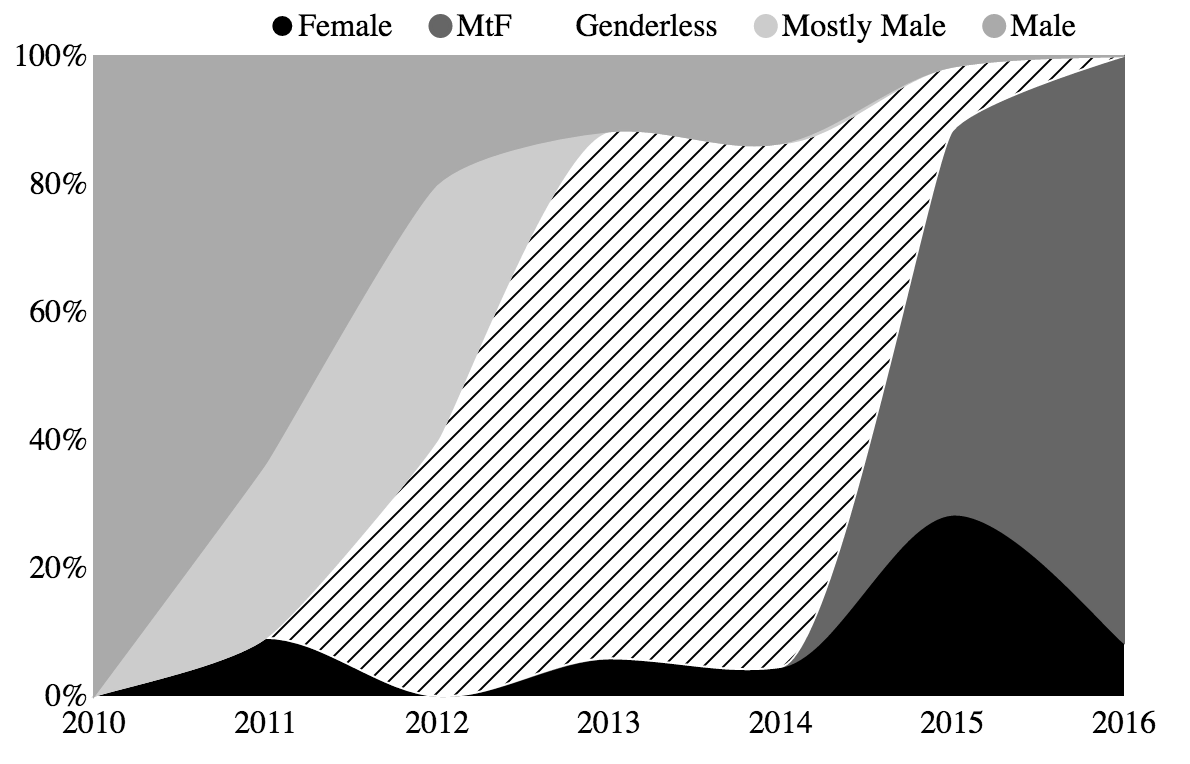
\includegraphics[scale=0.45]{assets/commissions-sex-preview.png}
  \caption{\textit{Gender expression of the author's character as portrayed in visual commissions over the years.}}
  \label{fig:commissions-sex}
\end{figure}

Figure \ref{fig:commissions-sex} shows the ways in which the sex of my characters in art that I commissioned changed over time.  There's a very clear trend from male to female, then from female (as an idealized form of myself) to a specifically trans fox (as I started to get comfortable with my identity as a transgender person).  I'm not alone in this progression, either, as many have found the utility in having a mostly safe space in which role-play is common and accepted behavior in which to explore various aspects of their identity.

There's a very good reason for this, too, but first, lets hear from another critter using furry as a lens to help in the explorations of their gender.

\secdiv

%%%%% Indi may not be able to take part
% \begin{center}
%   \textit{The intro is super rough and needs to be thoroughly reworked.}
% \end{center}
%
% Indi is many things.  We all are, of course, but ve is a wonderful example when it comes to building up the critter you want to be out of the things that are important to you.  Ve is most commonly a plush coyotter --- a coyote/otter hybrid in stuffed animal form --- covered in glowy markings in teal, purple, and green. Everything is chosen very deliberately.  Ver constituent species is each important to ver in its own way, as well as each of the colors chosen as\ldots{}tattoos?  Markings?  Shifting signifiers of emotion, attitude, and status.
%
% You see, this is why I love postfurries so much.  No other crowd that I've had the chance to spend time with has been so interested in self-actualization of so many portions of their identity.  Postfurry is a topic for another piece, but it's worth bringing up that Indi typifies the class: ve is doing ver best to find a way to not just emulate but become what ve feels verself to be, but to actually achieve that as ver reality.
%
% This naturally finds its way into the ways in which ve experiences, expresses, and talks about gender.  You've noticed the pronoun choices, surely --- ve/ver/vis --- but it's worth talking a little about how exactly Indi identifies, as well as how ve got there and how furry helped.

\secdiv

I just spent quite a few words talking about the genderful exploration of one critter and they way that it interacted with ver membership in the postfurry community, but these sentiments go far beyond just that small sector of furry.

I started a small, informal poll on twitter, and got inundated with responses.  The poll itself was simple:

\begin{quotation}
  Hi.

  Tell me about how furry helped you with figuring out your gender identity!

  Thanks.

  \textit{--- Tweet from @drab\_makyo on July 6, 2016}
\end{quotation}

The responses were overwhelmingly positive, though some had a few caveats.  Many said that the opportunity to create a character as an ideal form of themself offered them the possibility to find a way to be more true to more aspects of their identity than they might have had in the first place.  Furry, it seems, provides a constructive and creative place in order to explore.

You'll note, however, that I didn't say `safe place' above.  Many of the caveats to furry being a good place to explore gender surround the fact that, in a lot of ways, many folks who identify as trans or non-binary (as well as intersex folks) feel fetishized more often than not.  Gender, as we well know, goes far beyond just the interactions of genitalia.

Another caveat that I heard was that, although the subculture provided a healthy means to \textit{begin} exploring gender, many felt that the thing that helped them mature in their identity was seeing representation outside of the fandom, as well.  This was especially true for some of the non-binary folks that I got the chance to talk with.

There's much more that I can say on the matter of why furry might be good for exploration, and I will shortly, but first, there is far more data available than just a single twitter poll!  After all, as Executive Data Vix for [adjective][species], it's my job to administer the Furry Poll, the fandom's largest market survey, and then to go for deep dives into that giant pool of data.

To that end, I started pulling some numbers from the 2016 Furry Poll.  There were 3194 total responses to look at which were relevant to our topic at hand.  Here are the questions that we asked:

\begin{enumerate}
  \item What is your age in years?
  \item What best describes your gender identity?
  \begin{itemize}
    \item Masculine or mostly masculine
    \item Feminine or mostly feminine
    \item Other \textit{(NB: there were a series of options, including a write-in option, which, for our purposes, have been boiled down to an `other' category.)}
  \end{itemize}
  \item Does your gender identity now align with your sex as assigned at birth?
  \begin{itemize}
    \item Yes (I am cisgender)
    \item No (I am not cisgender)
    \item It's complicated (exactly what it says on the tin)
  \end{itemize}
\end{enumerate}

What all did we get?  Well, nothing too surprising, and let me explain why.

\begin{figure}
  \centering
  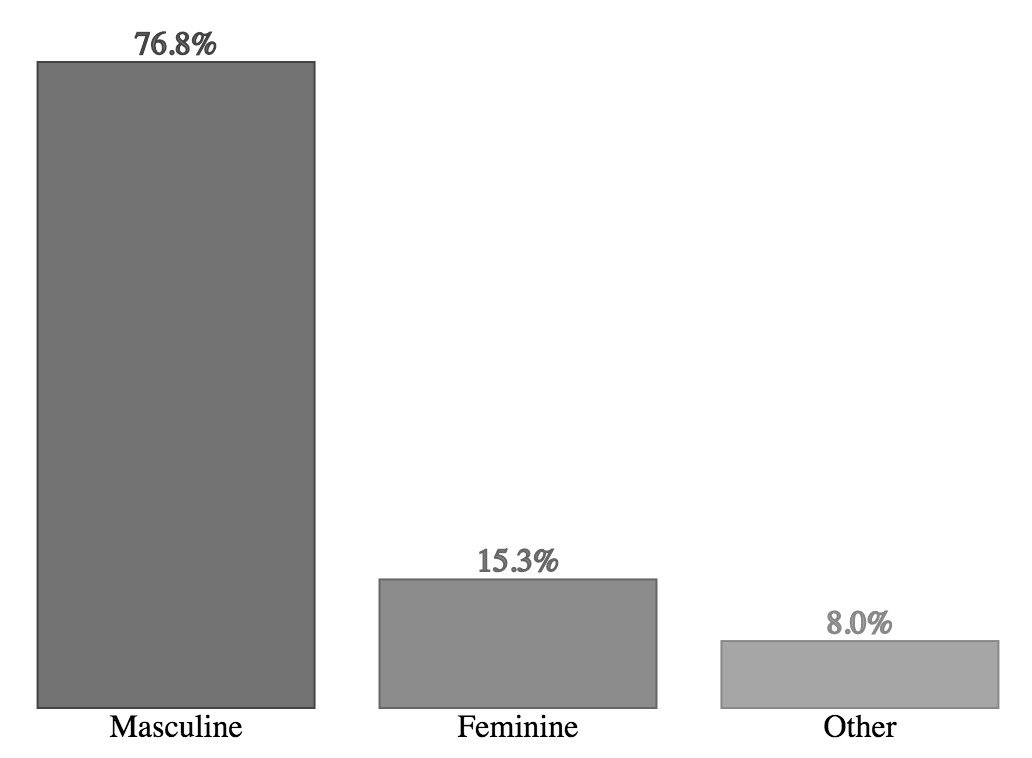
\includegraphics[scale=0.45]{assets/identity.png}
  \caption{\textit{Gender identity of respondents in the 2016 Furry Poll.}}
  \label{fig:identity}
\end{figure}

The ideas that we hold to be true without proof comprise our \textit{doxa}.  That is, the things we assume to be true, or to be the case, without needing to have anything backing those assumptions up.  When one looks around the furry fandom at time of writing, one is likely to find a subculture made up mostly of men.

To that, the survey offers only confirmation (fig. \ref{fig:identity}).  A bit more than 75\% of the respondents --- certainly a supermajority --- responded that their gender identity was masculine or mostly masculine.  Although one's expression or presentation used as a predictor has its flaws, a glance around the average convention space bears truth to this claim: we can mark that down as one point for doxa reading things correctly.

\begin{figure}
  \centering
  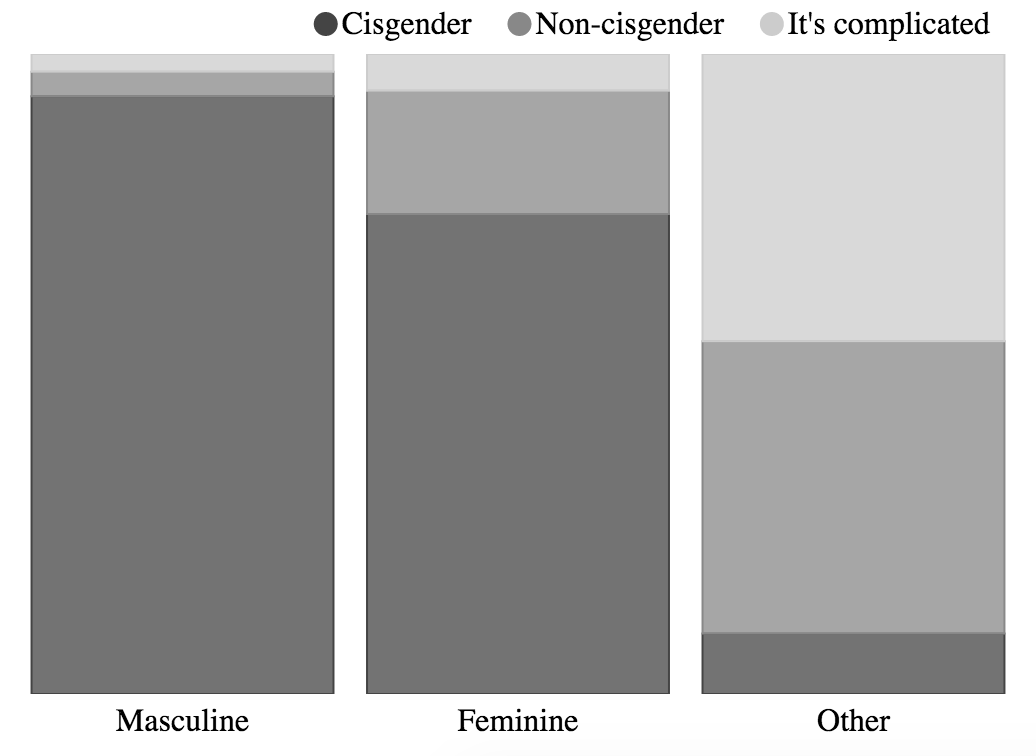
\includegraphics[scale=0.45]{assets/alignment.png}
  \caption{\textit{Gender alignment of respondents in the 2016 Furry Poll.}}
  \label{fig:alignment}
\end{figure}

Now, how about we look at gender alignment (fig. \ref{fig:alignment}); that is, let's take a look at the breakdown of how folks' gender identity aligns with their sex as assigned at birth.  For example, a trans man who was assigned female at birth, but identifies as a man now, would be someone who would fall under the umbrella term of `transgender', while a man who was assigned male at birth would fall under the term `cisgender'.  Additionally, for the sake of completeness, the survey also offered the choice for the respondent to answer that the answer was more complicated than these two choices would allow (we did not ask for further details, and had we, we would not be able to share them while preserving anonymity, of course).

\secdiv

\begin{center}
  \textit{Another story}
\end{center}

\secdiv

Given the stories of those exploring and expressing gender and identity through the framework of furry, the obvious next question that needs to be asked is ``why?''

Naturally, these sorts of things are not answered by any simple quip, nor even a single article like this.  That said, there are some things that we can point to that might help explain just why the furry subculture plays as big a role as it does in the formation of its members' identities, gender and otherwise.

There are a pair of twinned concepts within the realm of psychology that have been applied to this topic in particular.  Aaron Devor, a sociologist and dean of graduate studies at the University of Victoria in Canada, described them most succinctly in their paper, ``Witnessing and Mirroring: A Fourteen Stage Model of Transsexual Identity Formation.''

The stages themselves are interesting, of course.  They describe the path that a trans person might take as they work through the process of coming out, transitioning, and so on.  I'm not going to list them here, to save on ink --- the paper is free, easy to find legally online, and worth a read on its own.  I'd like to talk about the twinned concepts mentioned in the title instead, as they play a much more integral role when it comes to figuring out why furry might be a good place for so many to explore identity.

Witnessing is the idea that we gain something in the way of validation by having others see us as we see ourselves.  For someone who is solidifying the image of themselves as they feel others ought to see it, to have someone outside themselves perceive them along those lines is incredibly validating.  For trans women to called ma'am, or trans men to be able to use the men's room, or for non-binary folks to be referred to by their proper pronouns\ldots{}all of these things are a form of witnessing, and help to reinforce the individual's sense that they are doing what is best for their life.

To go along with that, mirroring is the idea that we gain validation by way of seeing others who are like us.  For folks in the early stages of transitioning, this comes both in the form of seeing other folks in the early stages --- the ``I can do it too'' effect --- as well as folks later on in the process --- the ``See, it can be done'' effect.  When we see something of ourselves reflected in others, it adds a bit of realism to something that might have once only been a fantasy.

Within my circle of friends, we talk of the `gender cascade'.

This goes far beyond just our little in-group.  Folks have often talked about the cascade, perhaps using terms such as `transplosion', or one news source's amusing choice of `transgender mania'.  In both cases --- either constrained by the constituents of a subculture or relatively unrestricted and part of society at large --- those who are questioning their gender, or even those who are certain but unsure of beginning transition, can gain validation through witnessing and mirroring.  That is, they can allow themselves to be seen as they are in safe contexts and see others who are like themselves in order to gain the confidence to move forward.

Furry provides fertile soil for this sort of thing due in large part to the fact that we explicitly design the image that others think of when they think of us, through the formation of our personal characters, avatars, or fursonas, however you want to think of it.

If you flip back to the graph of the sex of my characters that were represented in commissioned furry art, you can see a very definite shift away from male.  At first, I shifted from masculine to explicitly genderless, because my identity had become so painful to me that my instinct was to escape.  From there, as I gained confidence and with validation from others, I started to incorporate more and more feminine aspects into my characters.

Your character is an unspoken-yet-explicit way for a fur to say, ``This is how I ought to be seen.''  For trans folk, it provides a useful tool in terms of exploring gender identity: although mirroring becomes mudding in many circumstances (for those role-playing as a different gender, being outed as such isn't exactly desirable), it sure as hell makes witnessing easier.  I became a fox girl on the internet long before I got the letter that allowed me to start hormone replacement therapy.

There's a conclusion that I draw from all of this, though it took, me some time to connect the dots, pull it up, draw it all together, and many other metaphors.

When I started associating with animal people on the internet, I did so as a fragile teen who could barely admit that sex was a thing that existed, much less a being with a sexual orientation, never mind one that might not be straight, or even sexual.  Meeting and interacting with sexual, non-straight, and happy folk helped change that over the process of a few years, and a few halting relationships.

(Exes, if you're reading this, I don't apologize for being a gawky youth with awkward pretenses of sexuality, or for the late-night whining, but I will apologize for being a shit about the way things ended.)

Fast-forward a few years, and there I was: a mid-twenties person in the middle of an identity crisis.  What was I?  Was I nothing?  Sex was a panic-riddled minefield of unmet expectations and awkward feelings of being built wrong.  Was a I woman, with my my dreams of motherhood-but-not-fatherhood?  Was I something in between, with the fact that womanhood discomfited me in a different way than manhood?

Here, unlike with my orientation, I had enough experience to both look around me and see those going through something similar, as well as to take a step to be seen as who I felt that I might be.  I started out haltingly, and went down a few wrong paths (looking at you, plush phase; love me some plushies, but it's not me), but I found myself a niche.  It came in the form of a description and a few megabytes of graphical data culled from the minds and tablets of some artistically minded friends.  It led to me confronting my therapist one day and saying, ``Hey, can you write me a letter?''

Fast forward another year or two, and where am I?

I'm putting together the pieces of the fact that this isn't a uniquely trans thing, though this is an article on the intersection between gender and furry.  Neither is it a uniquely sexual thing, though the intersection between sex and furry is worth an article of its own.  It's something one layer up.  It's membership in a community that provides a mechanism and a place for these discoveries to take place.

Is it a uniquely furry thing?  Almost certainly not.  However, there's no doubt that furry played a rather large role in it for me, just as it did for so many other folks.

Without furry, I might just as well have come out as gay, then neutrois, then genderqueer, then trans, then all of those other wonderful labels.  But would I have felt safe doing so?  Would I have gotten all of the validation that I needed to feel healthy doing so?  Would I have come away with countless other brothers, sisters, and non-binary siblings in whom I could confide, admire, and rejoice?

I don't know.  I think not, though.
% expand this last section, ends too suddenly
